% !Mode:: "TeX:UTF-8"

\section{项目设计与实现}

\subsection{硬件设计}

\subsubsection{系统总体架构}
系统采用模块化设计，以STM32F103C8T6微控制器为核心，通过I2C和USART总线连接各外围模块，实现OLED显示、六轴运动传感、蓝牙通信与状态指示等关键功能。系统总体架构如图\ref{fig:watch_arch}所示，包含主控制器模块、OLED显示模块、MPU6050传感器模块、HC-05蓝牙模块和电源模块。

\begin{figure}[h]
    \centering
    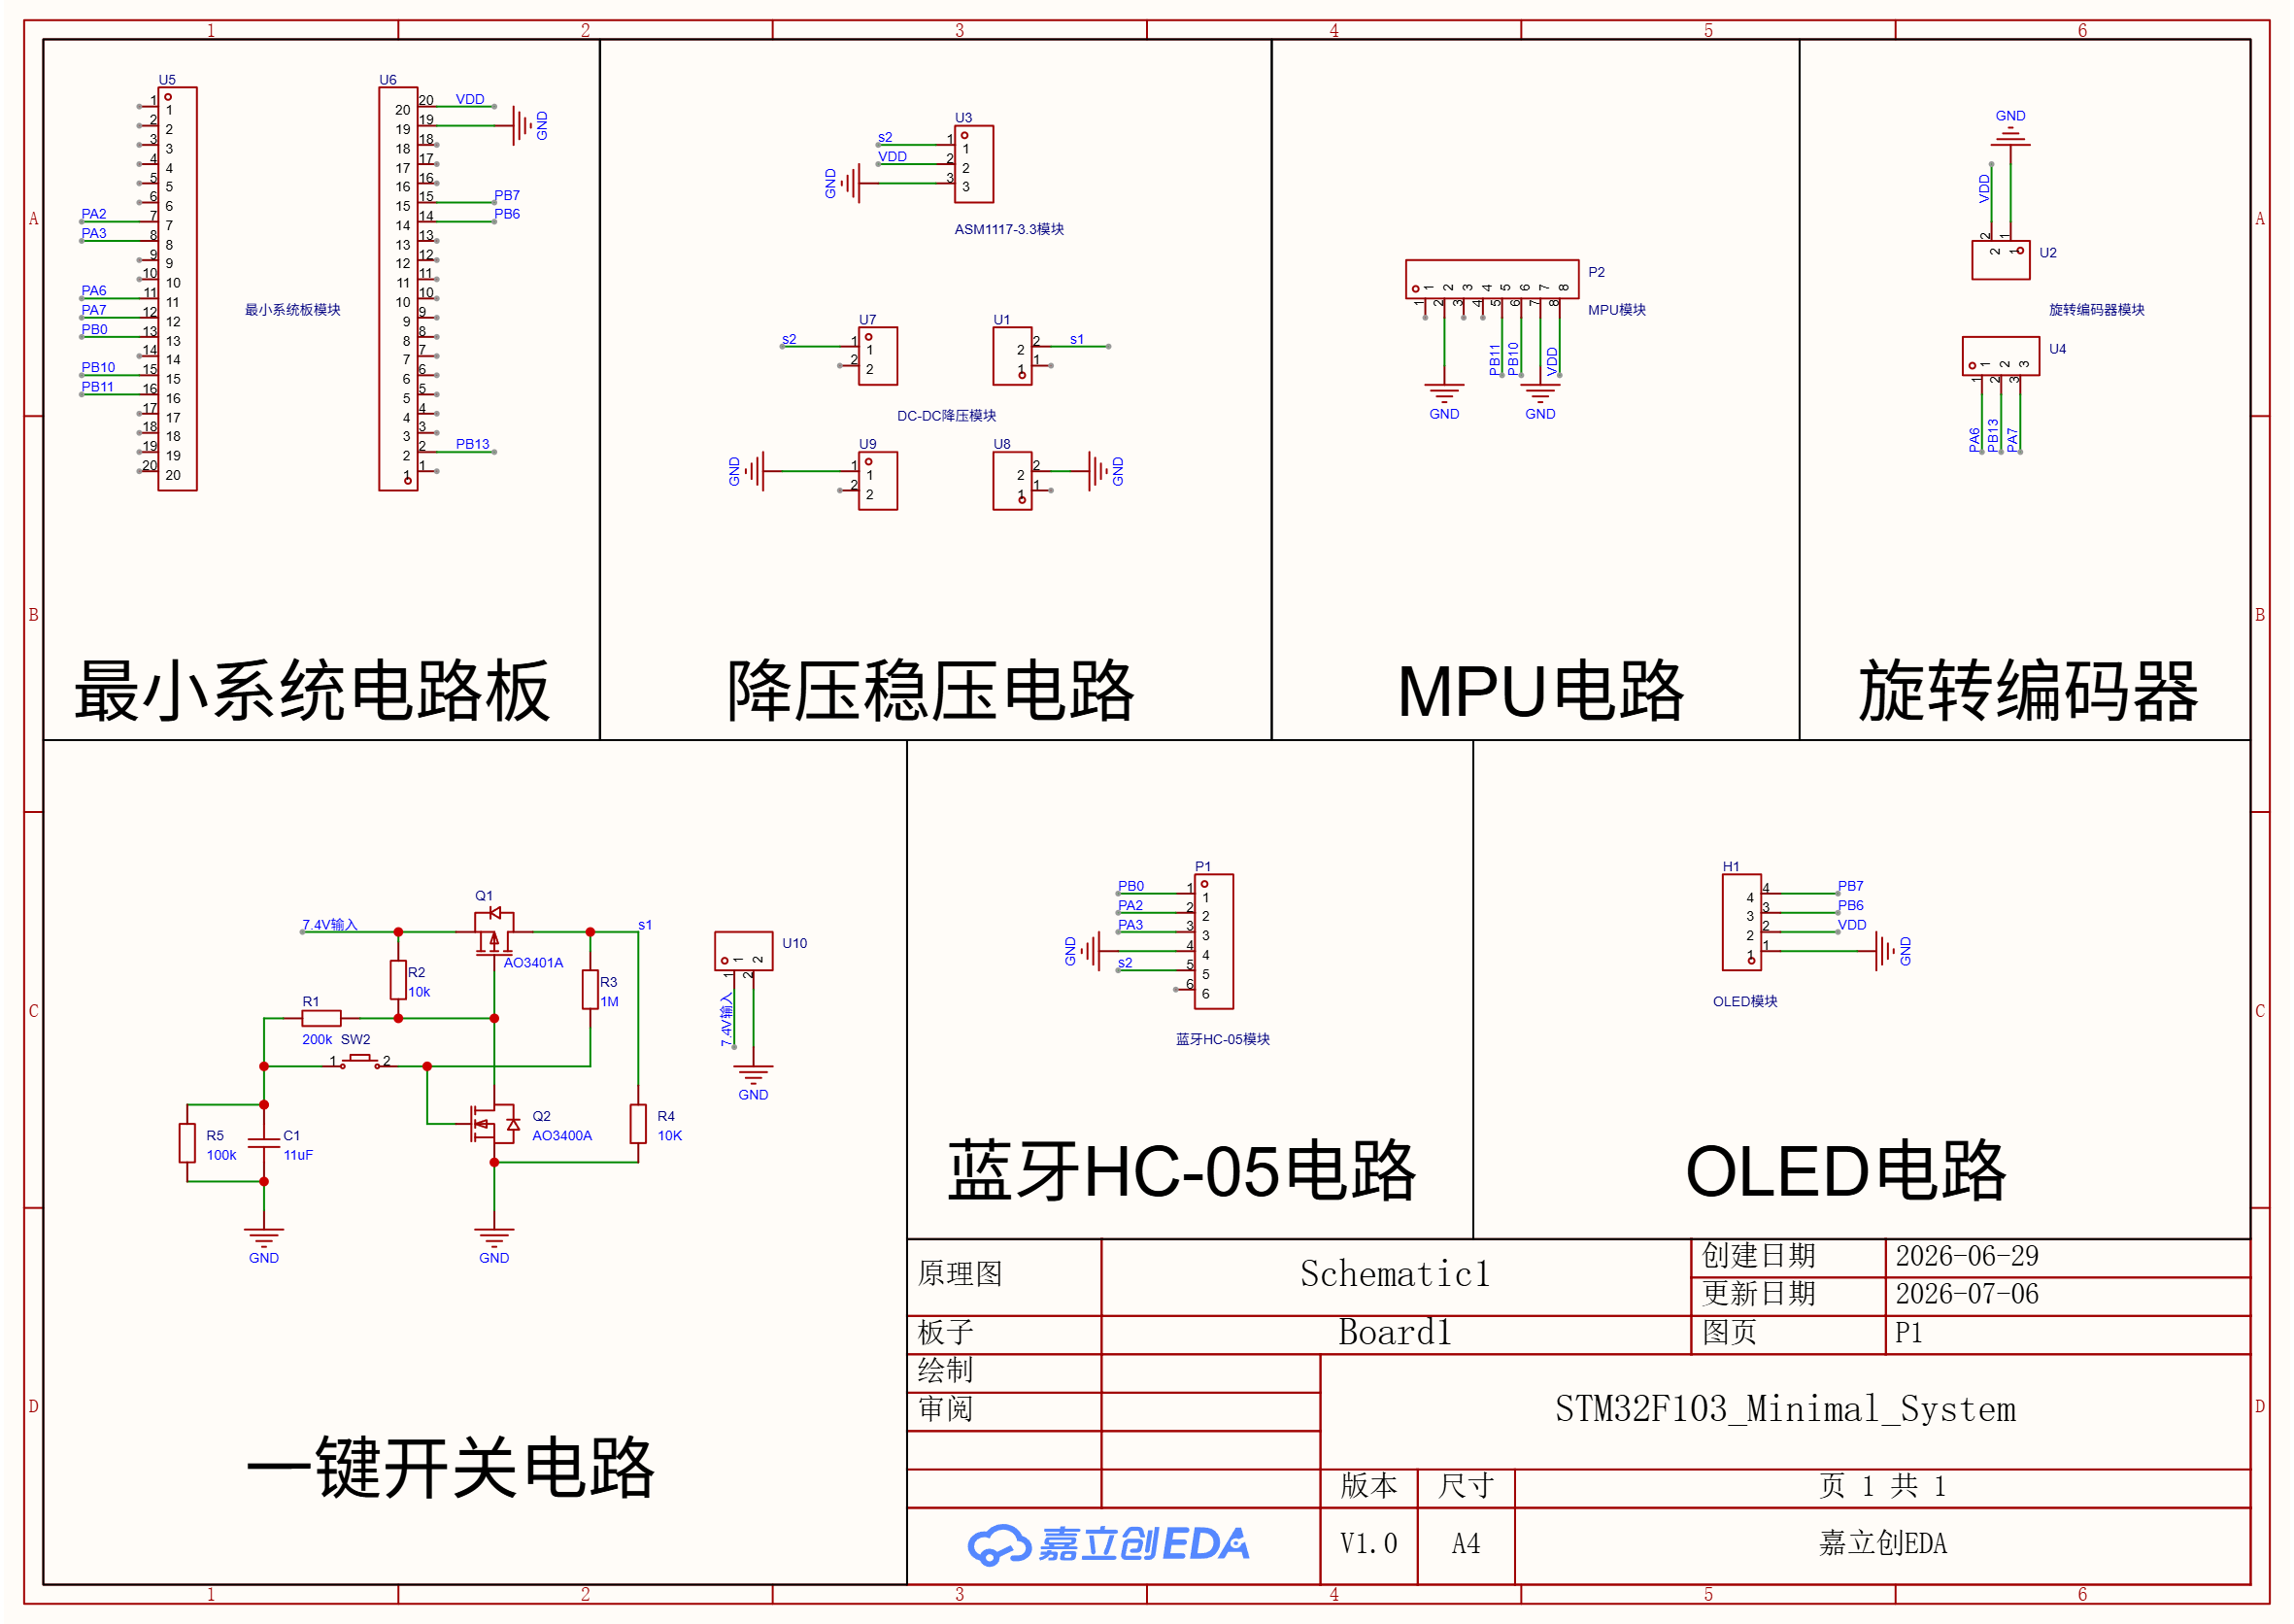
\includegraphics[width=0.9\textwidth]{figures/原理图终版.png}
    \caption{智能手表系统硬件原理图（STM32F103C8T6核心 + 多外设模块总线连接）}
    \label{fig:watch_arch}
\end{figure}

\FloatBarrier

\subsubsection{主控制器模块}
选用STM32F103C8T6微控制器作为主控芯片，主要特性包括：
\begin{itemize}
    \item 72MHz Cortex-M3内核，64KB Flash，20KB SRAM
    \item 2个I2C接口（I2C1用于OLED，I2C2用于MPU6050）
    \item 3个USART接口（USART2用于HC-05蓝牙）
    \item 4个通用定时器（TIM2用于软RTC秒中断）
    \item DMA控制器（用于USART2接收环形缓冲）
\end{itemize}

\subsubsection{OLED显示模块}
采用SSD1306驱动芯片的128$\times$64黄蓝双色OLED显示屏，主要特性：
\begin{itemize}
    \item 工作电压：3.3V
    \item 通信接口：I2C（地址0x3C，写操作0x78，读操作0x79）
    \item 引脚连接：SCL$\rightarrow$PB6，SDA$\rightarrow$PB7
    \item 显示模式：图形模式，支持像素级操作
    \item 页寻址模式：将128$\times$64显存分为8页（每页8行）
\end{itemize}

\subsubsection{MPU6050六轴传感器模块}
采用MPU6050六轴运动处理组件，主要特性：
\begin{itemize}
    \item 工作电压：3.3V
    \item 通信接口：I2C（地址0x68，写操作0xD0，读操作0xD1）
    \item 引脚连接：SCL$\rightarrow$PB10，SDA$\rightarrow$PB11
    \item 加速度量程：$\pm$2g（16384 LSB/g）
    \item 陀螺仪量程：$\pm$250°/s（131 LSB/°/s）
    \item 内置温度传感器和16位ADC
    \item WHO\_AM\_I寄存器（0x75）固定返回0x68，用于设备识别
\end{itemize}

\subsubsection{HC-05蓝牙模块}
采用经典蓝牙SPP协议模块HC-05，主要特性：
\begin{itemize}
    \item 工作电压：3.3V（VCC需接5V以获得最佳性能）
    \item 通信接口：USART2，波特率115200
    \item 引脚连接：TX$\rightarrow$PA3（USART2\_RX），RX$\rightarrow$PA2（USART2\_TX），STATE$\rightarrow$PB0
    \item STATE引脚：硬件检测连接状态，未连接为低电平，连接成功为高电平
    \item 默认设备名称：HC-05，可通过AT指令自定义
\end{itemize}

\subsubsection{电源模块}
设计单电源供电方案：
\begin{itemize}
    \item 主控电路：AMS1117-3.3V稳压芯片，输入5V$\rightarrow$输出3.3V
    \item 所有模块统一由3.3V或5V供电，简化电源管理
    \item USB接口提供5V调试电源，支持固件下载和串口调试
    \item 电源滤波：每个模块VCC引脚并联0.1$\mu$F陶瓷电容
\end{itemize}

\begin{figure}[h]
    \centering
    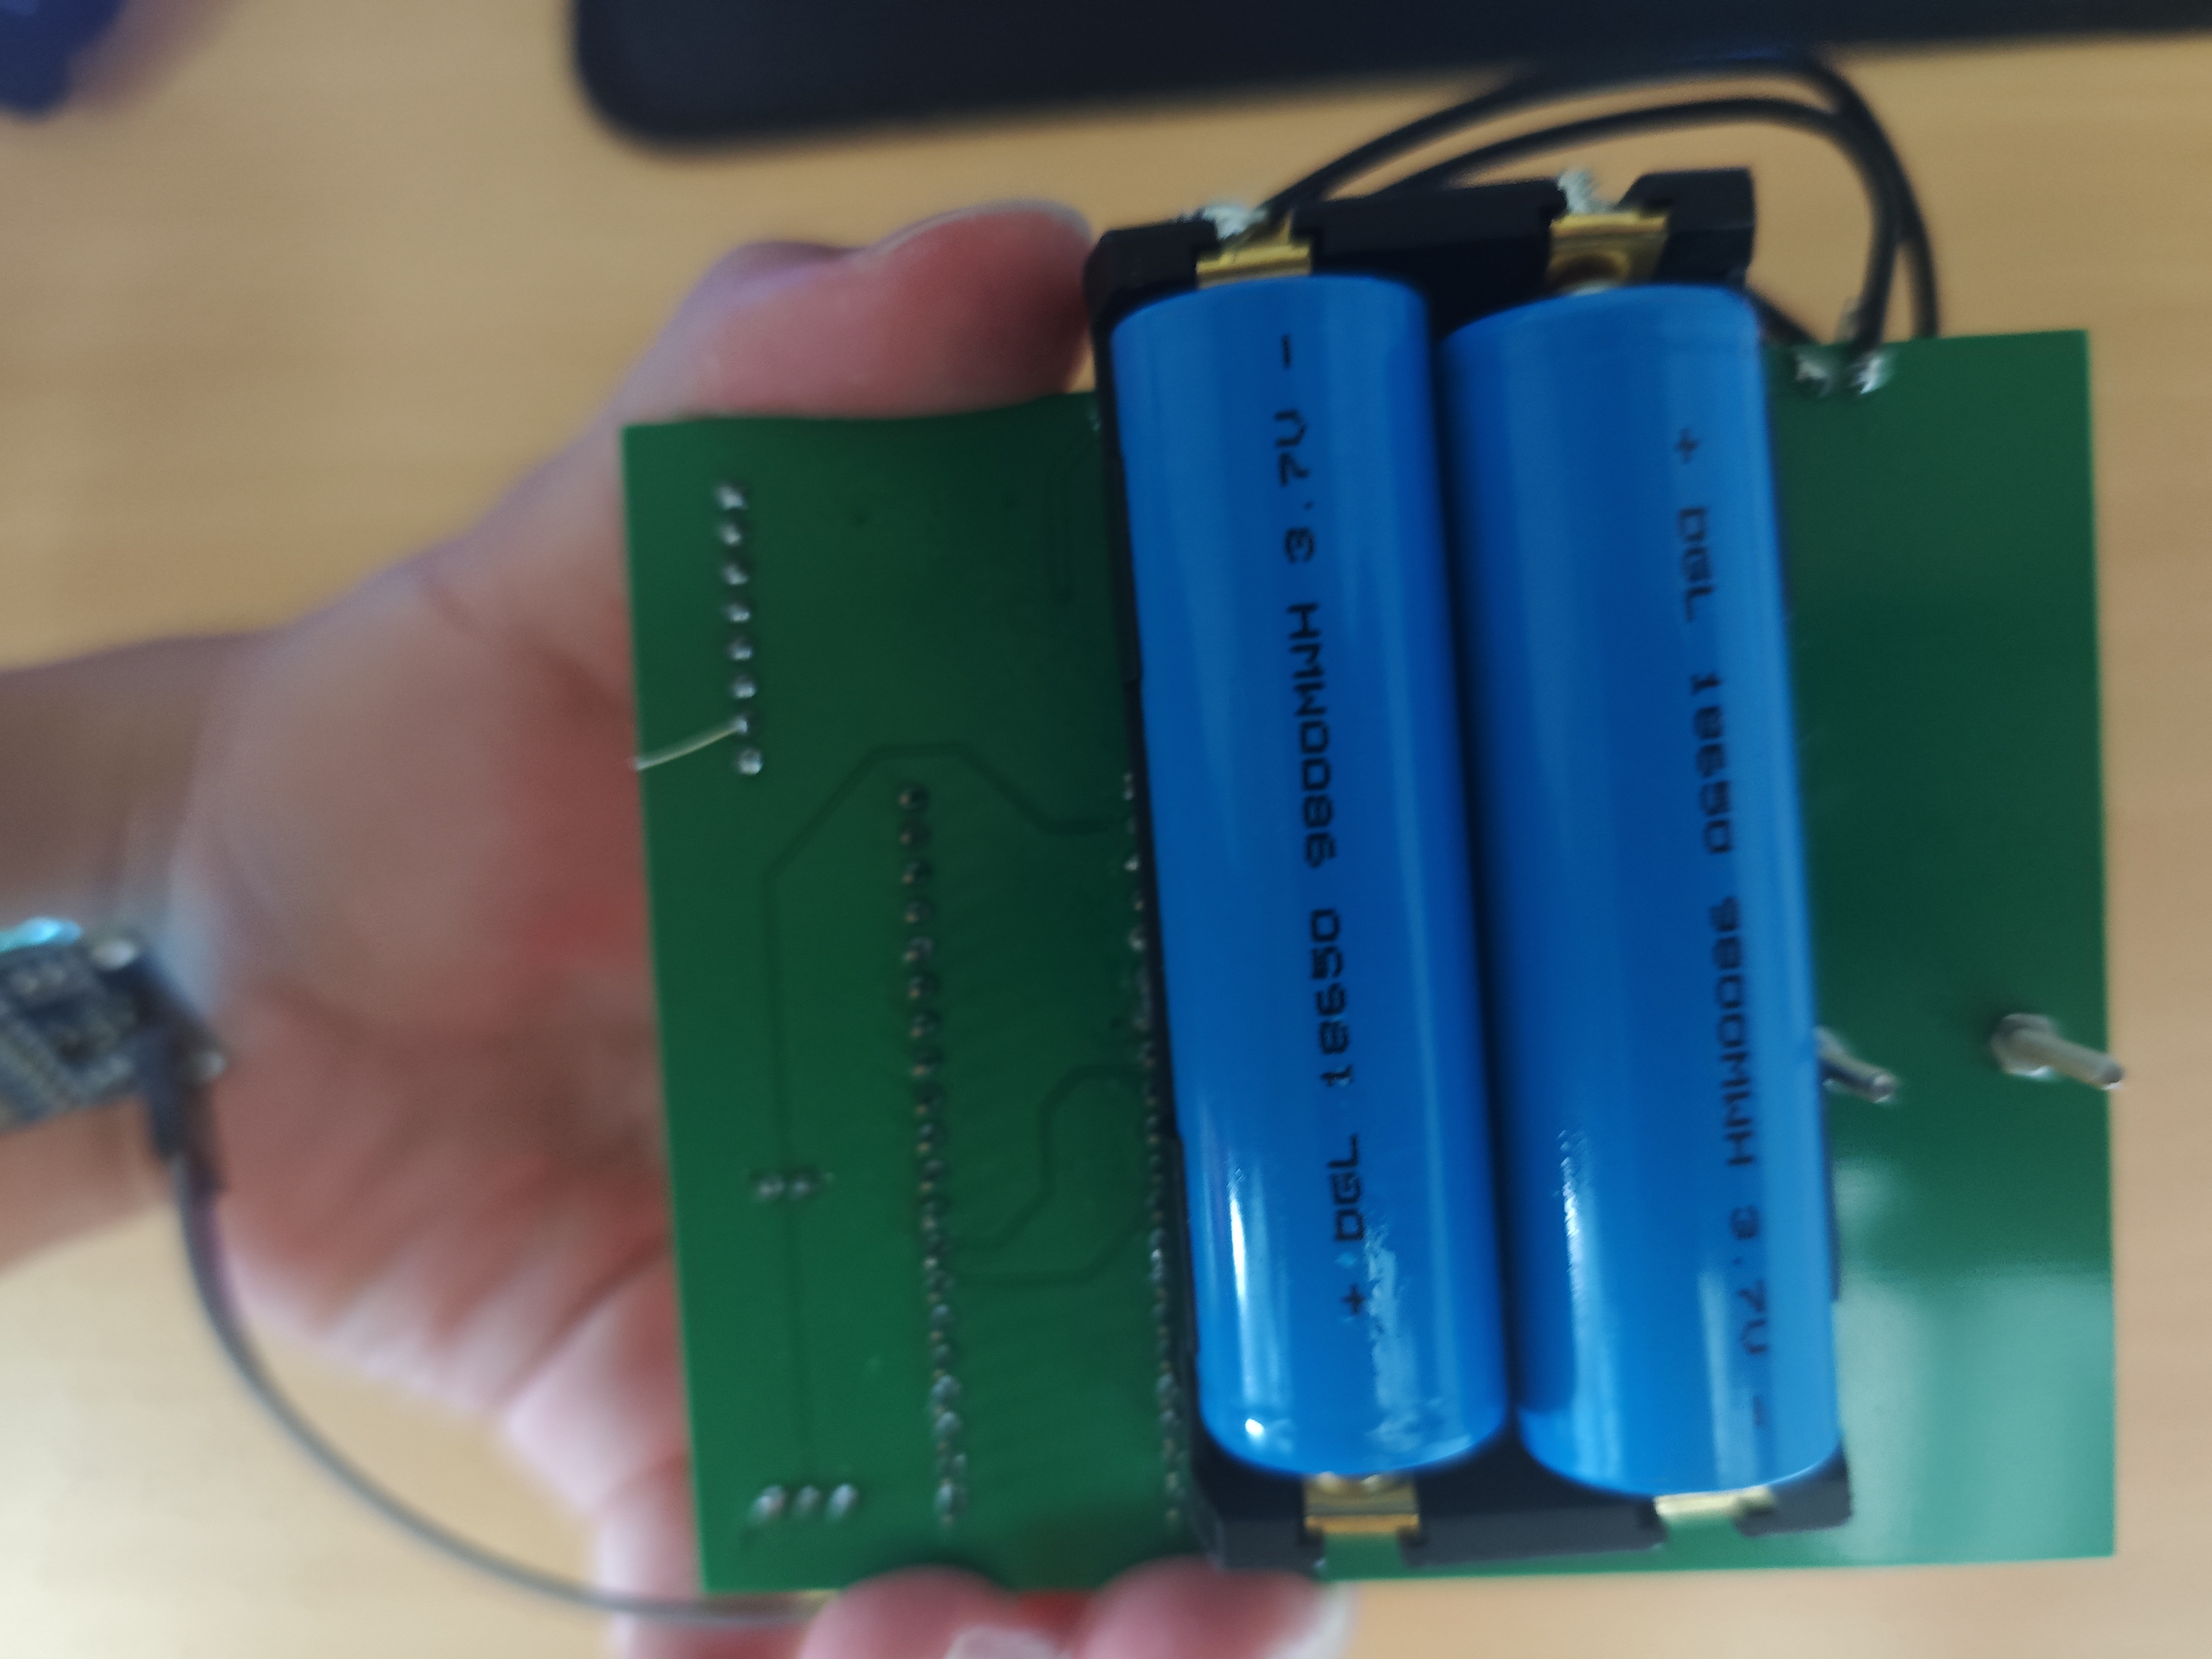
\includegraphics[width=0.5\textwidth]{figures/串联3.7V电池.jpg}
    \caption{电源模块实物图（串联3.7V电池供电方案，提供稳定5V/3.3V输出）}
    \label{fig:power_module}
\end{figure}

\FloatBarrier

\subsubsection{系统总体电路实物}
本系统所有模块在面包板上完成组装，核心模块通过杜邦线连接。STM32F103C8T6最小系统板位于中央，OLED显示模块和MPU6050传感器模块通过I2C总线连接，HC-05蓝牙模块通过USART2串口连接。系统总体电路实物如图\ref{fig:full_circuit}所示。

\begin{figure}[h]
    \centering
    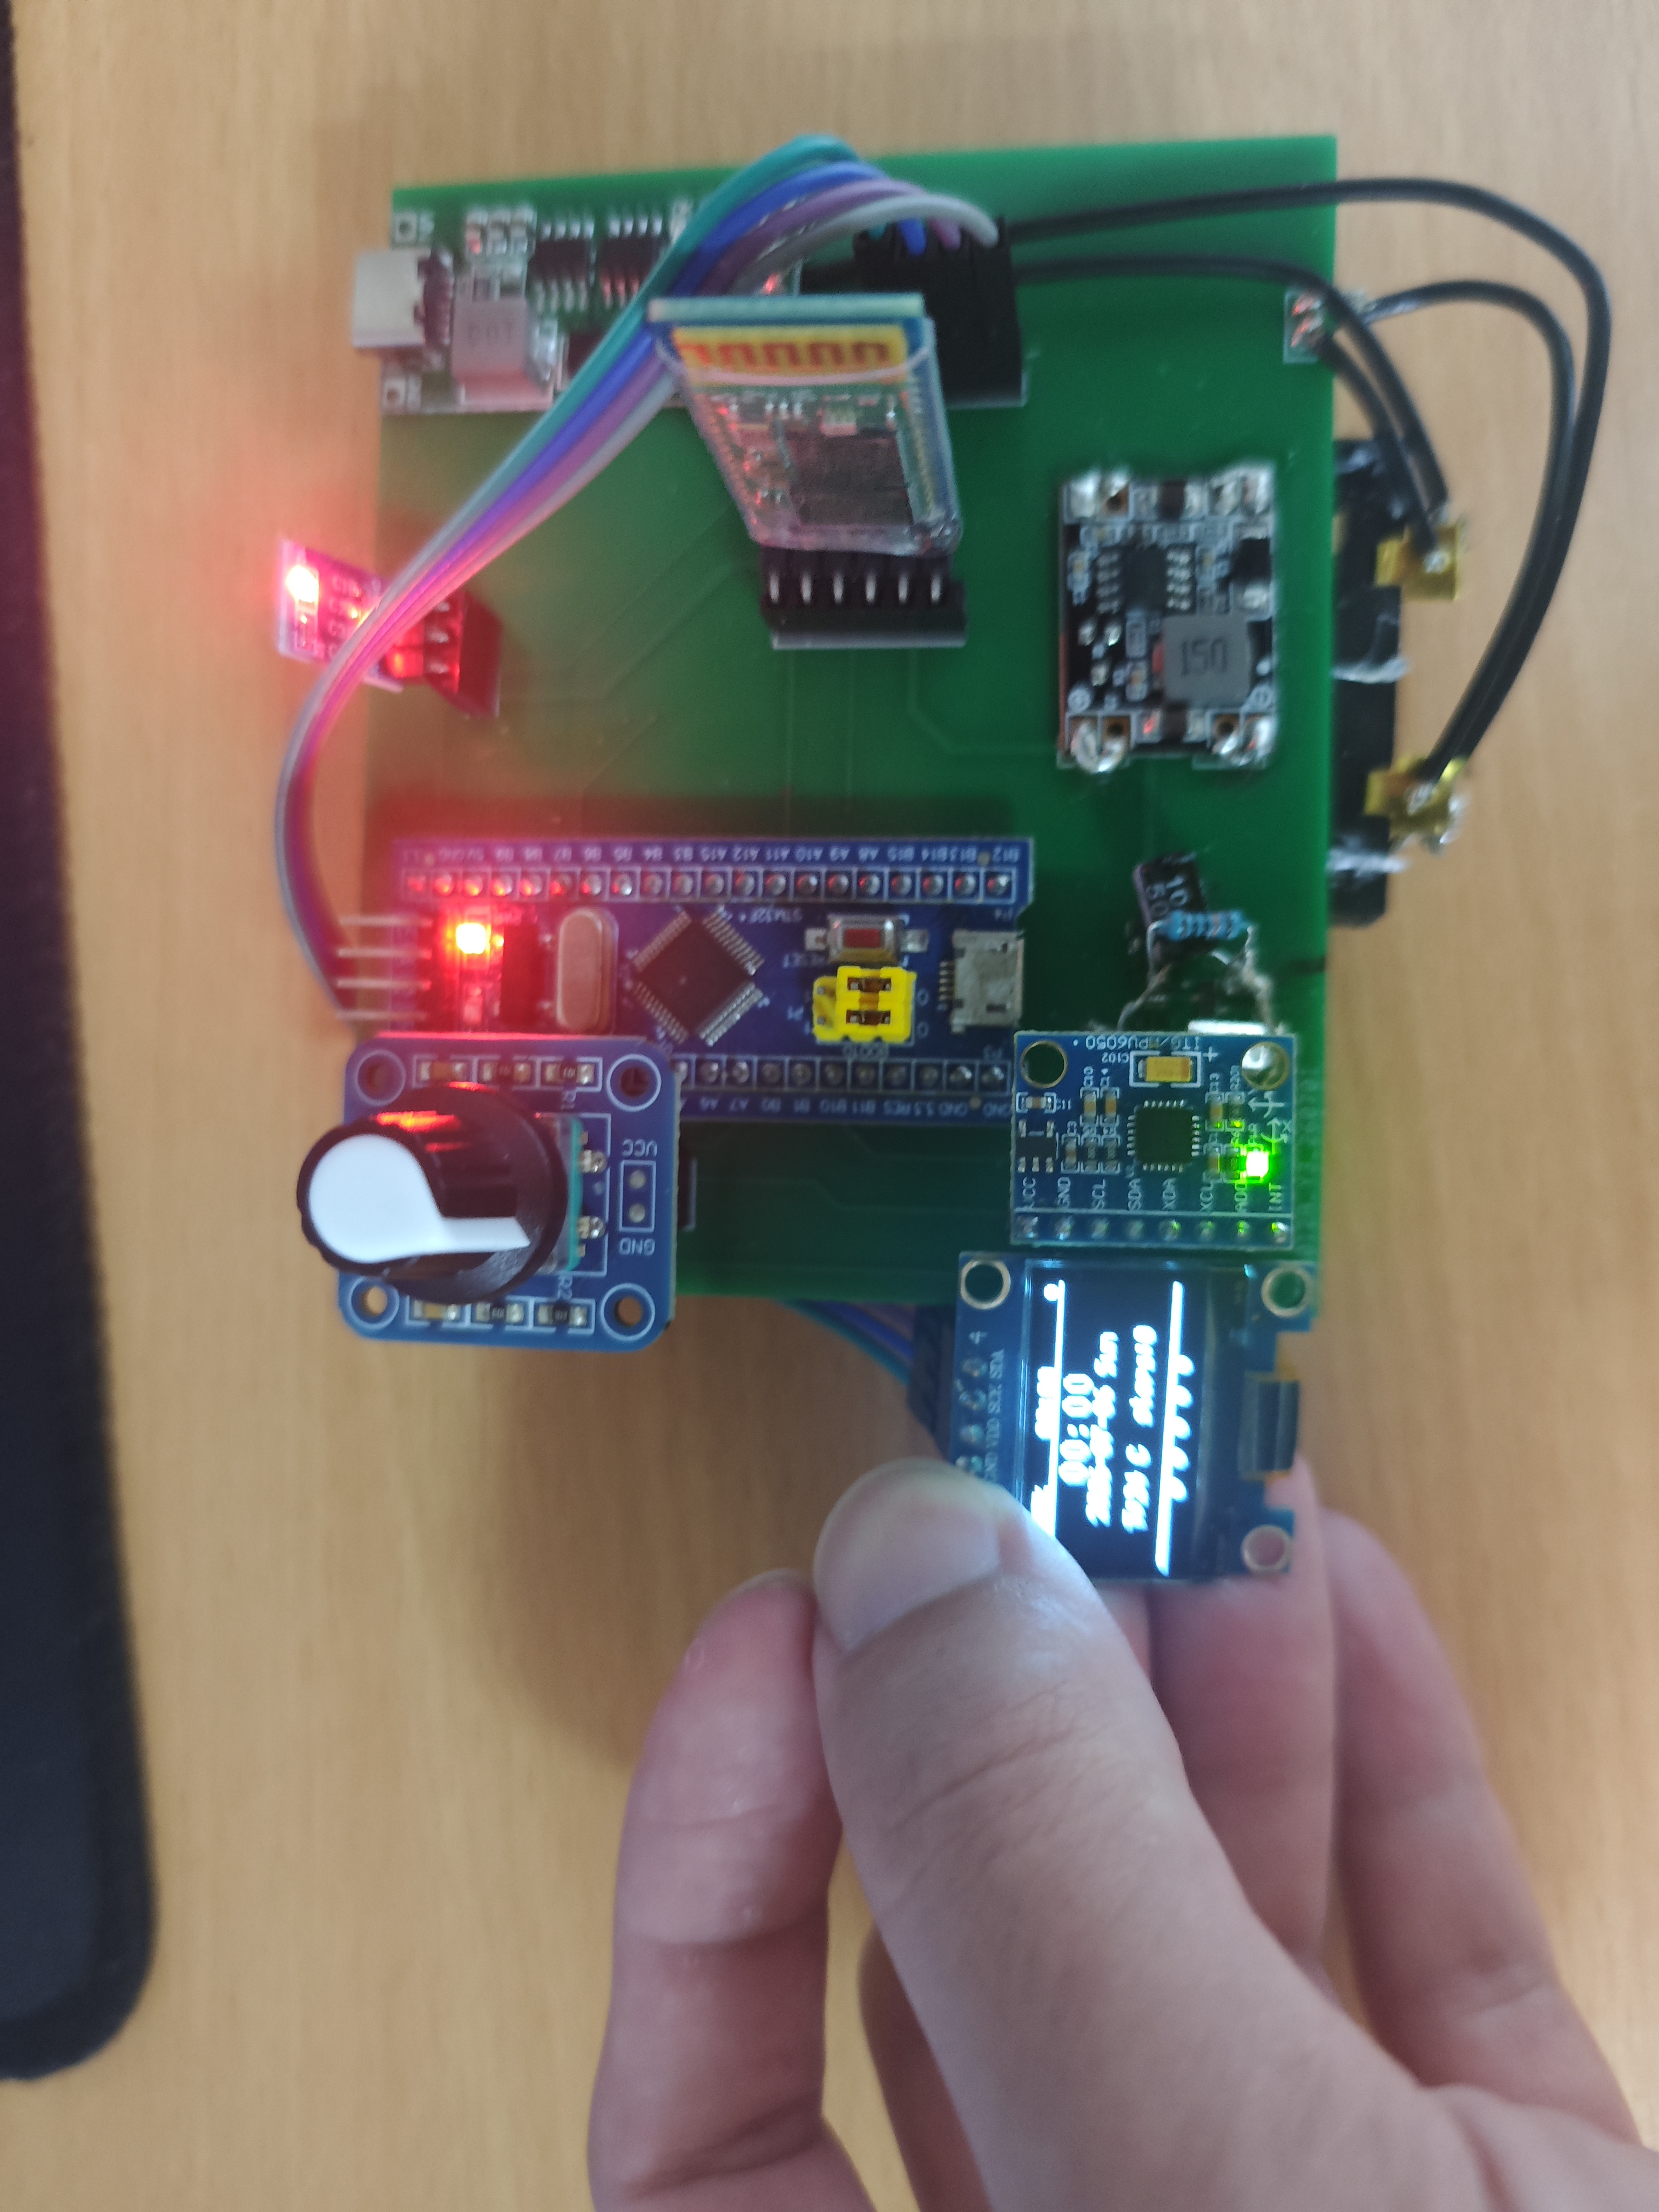
\includegraphics[width=0.9\textwidth]{figures/总体电路.jpg}
    \caption{系统总体电路实物图（STM32F103C8T6核心板 + OLED + MPU6050 + HC-05蓝牙模块）}
    \label{fig:full_circuit}
\end{figure}

\FloatBarrier

\subsubsection{引脚分配汇总}
系统各模块引脚分配如表\ref{tab:pins}所示：

\begin{table}[h]
    \centering
    \caption{系统引脚分配表}
    \label{tab:pins}
    \begin{tabular}{|l|l|l|}
        \hline
        \textbf{模块} & \textbf{引脚} & \textbf{功能} \\ \hline
        OLED（SSD1306） & PB6 / PB7 & I2C1\_SCL / I2C1\_SDA \\ \hline
        MPU6050 & PB10 / PB11 & I2C2\_SCL / I2C2\_SDA \\ \hline
        HC-05蓝牙 & PA2 / PA3 & USART2\_TX / USART2\_RX \\ \hline
        HC-05 STATE & PB0 & GPIO输入，检测连接状态 \\ \hline
        状态指示LED & PC13 & GPIO输出，系统运行指示 \\ \hline
    \end{tabular}
\end{table}

\subsection{软件设计}

\subsubsection{系统软件架构}
软件采用分层模块化设计，层次清晰、便于维护：
\begin{enumerate}
    \item \textbf{硬件抽象层（HAL）：} STM32CubeMX生成的初始化代码，包括I2C、USART、GPIO、定时器、DMA配置
    \item \textbf{驱动层：} OLED显示驱动（oled.c）、MPU6050传感器驱动（mpu6050.c）、蓝牙协议（bluetooth.c）、I2C总线恢复（i2c\_drv.c）
    \item \textbf{应用算法层：} 计步器算法（pedometer.c）、软RTC时钟（soft\_rtc.c）
    \item \textbf{UI框架层：} 智能手表UI框架（smartwatch\_ui.c），管理多页面渲染
    \item \textbf{主应用层：} 主循环逻辑、系统调度、状态管理（main.c）
\end{enumerate}

各软件层之间的调用关系自上而下，上层模块调用下层模块提供的接口函数，最终通过HAL驱动层与硬件交互。

\FloatBarrier

\subsubsection{主程序流程}
系统采用超级循环+中断驱动设计，主流程如下：
\begin{enumerate}
    \item 系统初始化（时钟、GPIO、I2C、USART、DMA、TIM2中断）
    \item I2C总线恢复：通过模拟SCL/SDA时钟脉冲解除从机死锁
    \item OLED初始化：发送初始化命令序列，清屏显示
    \item MPU6050初始化：配置量程，WHO\_AM\_I校验
    \item 蓝牙状态初始化：检测STATE引脚状态
    \item 进入主循环，执行周期任务：
    \begin{itemize}
        \item 读取MPU6050数据并更新计步器
        \item 更新OLED页面内容（每3秒切换页面）
        \item 处理蓝牙DMA接收缓冲区，解析帧协议
        \item 检测HC-05 STATE引脚，更新连接状态
        \item TIM2 1Hz中断递增RTC时钟
    \end{itemize}
\end{enumerate}

\FloatBarrier

\subsubsection{自定义蓝牙帧协议设计}
设计轻量级自定义帧协议，帧格式定义如表\ref{tab:frame}和图\ref{fig:frame_format}所示：

\begin{table}[h]
    \centering
    \caption{蓝牙帧协议字段定义}
    \label{tab:frame}
    \begin{tabular}{|l|c|l|}
        \hline
        \textbf{字段} & \textbf{字节数} & \textbf{说明} \\ \hline
        STX & 1 & 帧头固定0xAA \\ \hline
        CMD & 1 & 0x01=传感器数据上报；0x02=时间同步；0x03=计步数据 \\ \hline
        DATA & N & 载荷（传感器为6$\times$4字节小端float） \\ \hline
        CHK & 1 & CMD + DATA全部字节做XOR校验 \\ \hline
        ETX & 1 & 帧尾固定0x55 \\ \hline
    \end{tabular}
\end{table}

\begin{center}
    \resizebox{0.95\textwidth}{!}{
    \begin{tabular}{|c|c|c|c|c|}
      \hline
      STX (0xAA) & CMD & DATA (N bytes) & CHK (XOR) & ETX (0x55) \\
      \hline
    \end{tabular}
    }
    \captionof{figure}{蓝牙帧协议结构示意图}\label{fig:frame_format}
\end{center}

各命令类型数据载荷说明：
\begin{itemize}
    \item \textbf{命令0x01（传感器数据上报）：} 24字节数据 = ax(4) + ay(4) + az(4) + gx(4) + gy(4) + gz(4)，全部为IEEE 754单精度浮点小端格式
    \item \textbf{命令0x02（时间同步）：} 3字节数据 = 时(1) + 分(1) + 秒(1)，手机下发给手表更新RTC
    \item \textbf{命令0x03（计步数据）：} 12字节数据 = 步数(4字节uint32) + 距离米(4字节float) + 卡路里(4字节float)
\end{itemize}

\subsubsection{OLED多页面UI设计}
实现5个信息页面循环切换（每3秒翻页），页面内容设计如表\ref{tab:pages}所示：

\begin{table}[h]
    \centering
    \caption{OLED显示页面定义}
    \label{tab:pages}
    \begin{tabular}{|c|l|l|}
        \hline
        \textbf{页面编号} & \textbf{页面名称} & \textbf{显示内容} \\ \hline
        1 & 表盘主页 & 16$\times$24大字时钟（时:分:秒）+ 日期（年-月-日）+ Pitch/Roll姿态角 \\ \hline
        2 & 传感器数据 & 三轴加速度（m/s$^2$）+ 三轴陀螺仪（deg/s）+ 温度（°C） \\ \hline
        3 & 蓝牙状态 & 连接状态（已连接/未连接）+ 波特率(115200) + 硬件引脚信息 \\ \hline
        4 & 设备信息 & MCU型号(STM32F103C8T6) + Flash大小(64KB) + SRAM大小(20KB) + I2C总线分配 \\ \hline
        5 & 活动计步 & 当前步数 + 累计距离（米）+ 消耗卡路里（kcal）+ 今日活动时长 \\ \hline
    \end{tabular}
\end{table}

\subsubsection{计步器算法设计}
基于加速度向量幅值（AVM）的峰值检测算法，核心流程如下：
\begin{enumerate}
    \item 计算加速度向量幅值：$AVM = \sqrt{ax^2 + ay^2 + az^2}$
    \item 低通滤波：$filtered = \alpha \times filtered + (1-\alpha) \times AVM$，$\alpha$取0.7
    \item 动态阈值：维护滑动窗口内的最大值和最小值，阈值 = (max + min) / 2 + 偏移量
    \item 峰值检测：当filtered从低于阈值上升到高于阈值时标记一个候选步
    \item 防抖处理：两次有效步数间隔必须大于200ms，过滤噪声抖动
    \item 距离估算：距离 = 步数 $\times$ 平均步长（默认0.7米）
    \item 卡路里估算：卡路里 = 步数 $\times$ 0.04 kcal/步（经验值）
\end{enumerate}

\FloatBarrier

\subsection{代码介绍}

\subsubsection{初始化和配置}
\begin{itemize}
    \item \verb|MX_I2C1_Init()|：配置I2C1为标准模式（100kHz），用于OLED通信
    \item \verb|MX_I2C2_Init()|：配置I2C2为标准模式（100kHz），用于MPU6050通信
    \item \verb|MX_USART2_UART_Init()|：配置USART2为115200波特率，启用DMA接收
    \item \verb|MX_TIM2_Init()|：配置TIM2为1Hz周期中断，用于软RTC时钟
    \item \verb|OLED_Init()|：发送SSD1306初始化命令序列，配置显示参数
    \item \verb|MPU6050_Init()|：配置加速度和陀螺仪量程，校验WHO\_AM\_I寄存器
    \item \verb|I2C_Bus_Recovery()|：通过模拟时钟脉冲执行I2C总线恢复
\end{itemize}

\subsubsection{主功能实现}
\begin{itemize}
    \item \verb|OLED_Show_String(uint16_t x, uint16_t y, uint8_t *str, uint8_t size)|：OLED字符串显示
    \item \verb|OLED_Show_Num(uint16_t x, uint16_t y, uint32_t num, uint8_t len, uint8_t size)|：OLED数字显示
    \item \verb|OLED_Draw_Big_Clock(uint8_t hour, uint8_t minute, uint8_t second)|：绘制16$\times$24大字时钟
    \item \verb|MPU6050_Read_Accel(float *ax, float *ay, float *az)|：读取并转换加速度数据
    \item \verb|MPU6050_Read_Gyro(float *gx, float *gy, float *gz)|：读取并转换陀螺仪数据
    \item \verb|MPU6050_Get_Temperature(float *temp)|：读取温度数据
    \item \verb|Bluetooth_Send_Frame(uint8_t cmd, uint8_t *data, uint16_t len)|：组装并发送蓝牙数据帧
    \item \verb|Bluetooth_Parse_Frame(uint8_t *buf, uint16_t len)|：解析蓝牙接收帧
    \item \verb|Pedometer_Update(float ax, float ay, float az)|：更新计步器状态，返回是否新一步
    \item \verb|Soft_RTC_Handler()|：TIM2中断回调，递增时/分/秒变量
    \item \verb|SmartWatch_UI_Render(uint8_t page)|：渲染指定编号的UI页面
\end{itemize}

\subsubsection{中断与回调}
\begin{itemize}
    \item \verb|HAL_TIM_PeriodElapsedCallback(TIM_HandleTypeDef *htim)|：TIM2周期中断回调，更新RTC时钟
    \item \verb|USART2_IRQHandler()| + DMA空闲检测：处理蓝牙环形缓冲接收
    \item 主循环中每100ms轮询MPU6050数据，每3秒切换OLED页面
\end{itemize}

\subsubsection{循环体结构}
\begin{verbatim}
while (1) {
  /* 1. 读取传感器数据 */
  MPU6050_Read_Accel(&ax, &ay, &az);
  MPU6050_Read_Gyro(&gx, &gy, &gz);
  Pedometer_Update(ax, ay, az);

  /* 2. 处理蓝牙数据 */
  if (dma_buffer_has_data()) {
    Bluetooth_Parse_Frame(rx_buf, rx_len);
  }

  /* 3. 定时上报数据（连接状态） */
  if (bluetooth_connected && report_timer_expired) {
    Bluetooth_Send_Frame(0x01, sensor_data, 24);
  }

  /* 4. 更新OLED显示（每3秒切换页面） */
  if (page_switch_timer_expired) {
    current_page = (current_page + 1) % 5;
  }
  SmartWatch_UI_Render(current_page);

  HAL_Delay(100);
}
\end{verbatim}

\subsection{技术实现细节}

\subsubsection{OLED驱动实现细节}
SSD1306采用页寻址模式，将128$\times$64像素显存分为8页（每页8行），驱动核心流程：
\begin{enumerate}
    \item 初始化阶段：发送配置命令（关闭显示、设置时钟分频、设置多路复用率、设置显示偏移、设置起始行、电荷泵设置、内存寻址模式、段重映射、COM输出扫描方向、COM引脚配置、对比度设置、预充电周期、VCOMH设置、全局显示开启、正常显示模式）
    \item 字符显示：使用预生成的字模数组（6$\times$8基础字模、8$\times$16标准字模、16$\times$24大字字模），按字节写入对应页的GDDRAM
    \item 像素绘图：计算像素所在页(page = y / 8)和位偏移(bit = y \% 8)，通过读-改-写操作更新单个像素
    \item 页面管理：每3秒切换页面索引，调用对应渲染函数重绘整屏
\end{enumerate}

\subsubsection{MPU6050数据读取与转换}
MPU6050传感器数据处理流程：
\begin{enumerate}
    \item 通过I2C读取0x3B-0x48共14字节寄存器数据（加速度、温度、陀螺仪）
    \item 组合高低字节为16位有符号整数（高字节在前，大端格式）
    \item 加速度除以16384.0得到以g为单位的数值，再乘以9.8转换为m/s$^2$
    \item 陀螺仪除以131.0得到以deg/s为单位的数值
    \item 温度转换公式：Temperature = (temp\_raw / 340.0) + 36.53
    \item 姿态角计算：Pitch = atan2(ay, az) $\times$ 180 / $\pi$，Roll = atan2(-ax, az) $\times$ 180 / $\pi$
    \item 错误检测：WHO\_AM\_I寄存器校验失败或I2C通信超时，标记传感器离线，每3秒尝试重连
\end{enumerate}

\subsubsection{蓝牙DMA环形缓冲实现}
为保证蓝牙通信的实时性和可靠性，采用DMA+空闲中断的环形缓冲方案：
\begin{enumerate}
    \item 配置USART2的DMA接收通道，设置环形缓冲大小为256字节
    \item 启用USART空闲中断（IDLE flag），在一帧数据接收完成时触发中断
    \item 中断服务程序中计算本次接收的数据长度（通过DMA计数器差值）
    \item 将数据从DMA缓冲区复制到应用层处理缓冲区
    \item 应用层按帧协议解析：搜索STX(0xAA)$\rightarrow$读取CMD$\rightarrow$读取DATA至ETX(0x55)$\rightarrow$校验XOR
    \item 发送流程：组装完整帧后，通过HAL\_UART\_Transmit()阻塞发送（短帧可接受）
\end{enumerate}

\subsubsection{I2C总线恢复机制}
为防止I2C从机处于死锁状态（SDA被拉低无法释放），在系统初始化阶段执行总线恢复：
\begin{enumerate}
    \item 将SCL和SDA引脚配置为GPIO输出模式
    \item 循环产生9个SCL时钟脉冲（每个脉冲约5$\mu$s高电平+5$\mu$s低电平）
    \item 在SCL空闲期间检测SDA是否被释放（高电平）
    \item 发送STOP信号（SCL低$\rightarrow$高，SDA低$\rightarrow$高）
    \item 重新配置SCL/SDA为I2C外设功能
    \item 确保OLED和MPU6050在初始化前处于可通信状态
\end{enumerate}

\subsubsection{软RTC时钟实现}
由于STM32F103C8T6无内置RTC（或未外接32.768kHz晶振），采用TIM2定时器模拟RTC：
\begin{enumerate}
    \item 配置TIM2为1Hz周期中断（72MHz系统时钟经预分频和自动重载寄存器配置）
    \item 中断服务程序中维护全局变量：秒、分、时、日、月、年
    \item 实现进位逻辑：秒满60进位分，分满60进位时，时满24进位日，日期根据月份和闰年处理
    \item 蓝牙接收到0x02时间同步命令时，直接更新时/分/秒变量
    \item OLED表盘页面从全局变量读取时间信息进行渲染
\end{enumerate}